\chapter{Speckle y procesamiento}

Esta clase tiene como objetivo comprender los pasos básicos para procesar imágenes radar. Para ello se descargarán imágenes de la web y se procesarán a distintos niveles de correcciones geométricas y radiométricas para poder luego visualizarlas.

\section{Descarga de imágenes}

Para descargar imágenes SAR utilizaremos el catálogo del \href{https://vertex.daac.asf.alaska.edu/}{Alaska Satellite Facility}\footnote{\href{https://vertex.daac.asf.alaska.edu/}{https://vertex.daac.asf.alaska.edu/}}. Diríjase a la página y en la sección de \texttt{Geographic Region} seleccione un área que incluya a la ciudad de Ushuaia (Figura \ref{fig:region}).

\begin{figure}[h!]
    \centering
    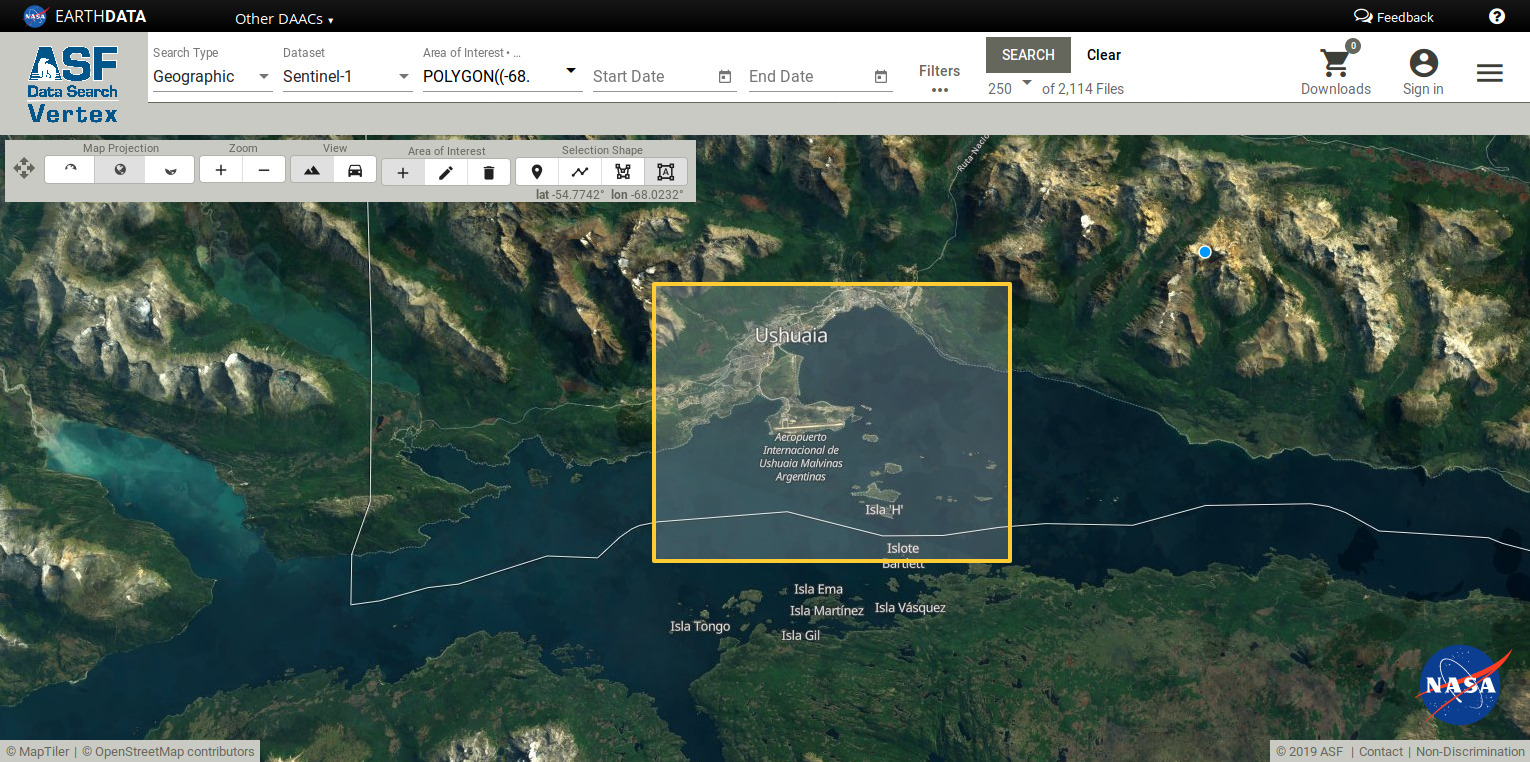
\includegraphics[width=0.9\textwidth]{fig:region.jpg}
    \caption{Selección de un área de interés en el catálogo \emph{Vertex} del \emph{Alaska Satellite Facility}}
    \label{fig:region}
\end{figure}

Seleccione en \texttt{Dataset} el set de datos de \texttt{ALOS PALSAR} (Figura \ref{fig:dataset}) y presione search.

\begin{figure}[h!]
    \centering
    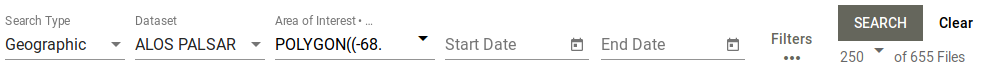
\includegraphics[width=0.9\textwidth]{fig:dataset.png}
    \caption{Selección de \emph{Dataset} en el catálogo \emph{Vertex} del \emph{Alaska Satellite Facility}}
    \label{fig:dataset}
\end{figure}

A la derecha de la pantalla aparecerá una lista de productos. Seleccione de ellos el de nombre \emph{ALOS PALSAR PLR} del 20 de abril del 2011, pertenenciente al frame 6070 y el path 119.

Descarge el producto \emph{Level 1.1 Complex (630.78 MB)} (Figura \ref{fig:descarga}). En caso de que el sistema así se lo pida, regístrese.

\begin{figure}[h!]
    \centering
    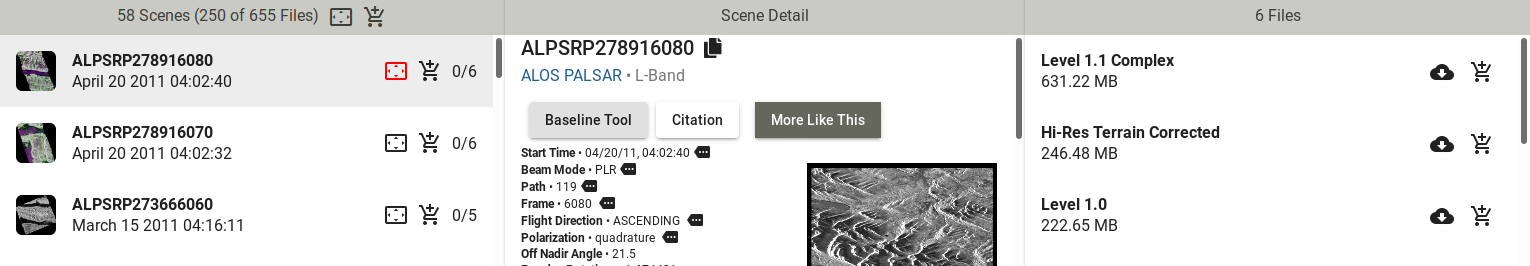
\includegraphics[width=0.9\textwidth]{fig:resultados.png}
    \caption{Selección de producto para la descarga en el catálogo \emph{Vertex} del \emph{Alaska Satellite Facility}}
    \label{fig:descarga}
\end{figure}

El producto descargado corresponde a una imagen \emph{Single look complex} en \emph{slant range}.

\section{Calibración}

Abra la imagen \directory{ALPSRP278916070-L1.1.zip} en SNAP. Despliegue la banda \texttt{intensity\_HH} y observe que se encuentra comprimida horizontalmente.

\begin{figure}[h!]
    \centering
    \subfloat[I/O Parameters]{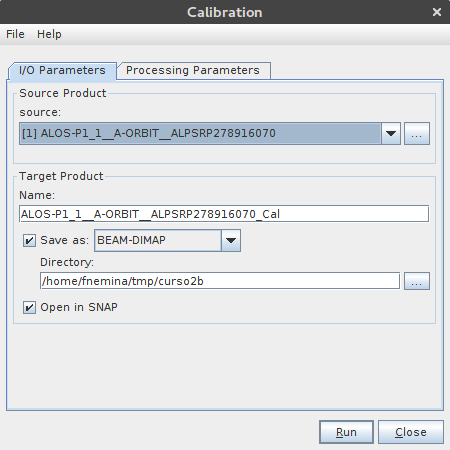
\includegraphics[width=0.35\textwidth]{fig:calibrar1.png}}
    \hspace{1cm}
    \subfloat[Processing parameters]{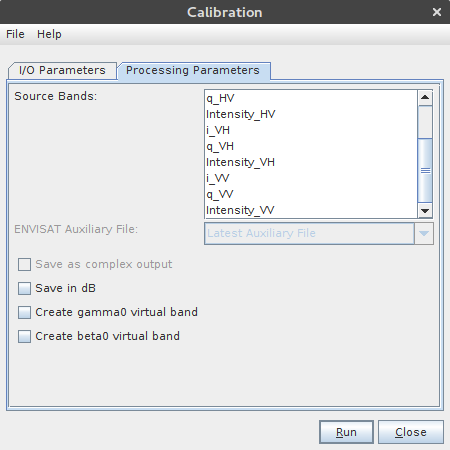
\includegraphics[width=0.35\textwidth]{fig:calibrar2.png}}
    \caption{Calibración de productos SAR utilizando el SNAP. Recuerde seleccionar la ruta de guardado en \emph{Directory}.} % arreglar figura
    \label{fig:calibrar}
\end{figure}

Para calibrar la imagen, diríjase a \menu{Radar>Radiometric>Calibrate} (Figura \ref{fig:calibrar}) y asigne una ruta de guardado.

 Obtendrá una imagen con los coeficientes de backscatter \texttt{sigma\_0}. En este caso tendrá las bandas correspondientes a las 4 formas de interacción entre el blanco y la radiación (HH, HV, VH y VV). Este tema será desarrollado en la próxima clase.

 \section{Filtrado}

 Para disminuir el ruido speckle en la imagen utilizaremos el proceso de multilook. El multilooking genera una nueva imagen a partir de los píxeles en una ventana. Para realizarlo utilice la herramienta \menu{Radar>SAR Utilities>Multilooking}.

 En \texttt{source} seleccione la imagen
 \begin{center} \texttt{ALOS-P1\_1\_\_A-ORBIT\_\_ALPSRP278916070\_Cal} \end{center}
 que generó en el paso anterior. La solapa Processing Parameters permite indicar el numero de looks y sobre que bandas se ejecutará; de no seleccionar ninguna, el proceso se realizará sobre todas las bandas. En este caso utilice 1 look y la totalidad de las bandas de la imagen (Figura \ref{fig:multilook}).

\begin{figure}[h!]
    \centering
    \subfloat[I/O Parameters]{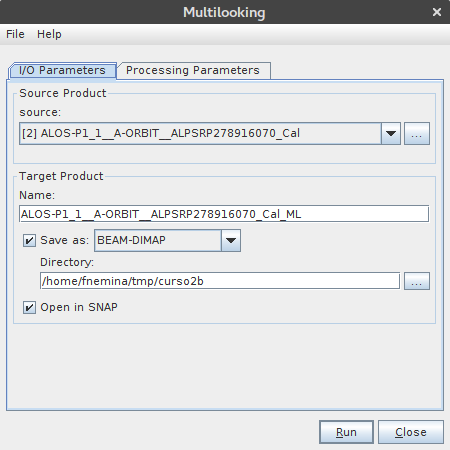
\includegraphics[width=0.35\textwidth]{fig:multilook1.png}}
    \hspace{1cm}
    \subfloat[Processing parameters]{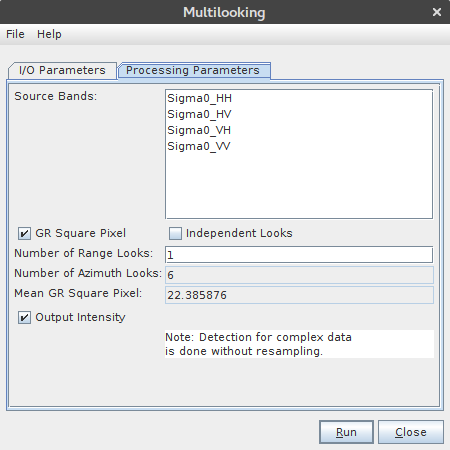
\includegraphics[width=0.35\textwidth]{fig:multilook2.png}}
    \caption{Multilook de una imagen SAR utilizando el SNAP.}
    \label{fig:multilook}
\end{figure}


\section{Proyección}\label{sec:proyeccion}

Finalmente, es común proyectar la imagen del \emph{slant range} al \emph{ground range}, para que luego se pueda abrir en cualquier softwarae de GIS sin problemas. Existen dos opciones: proyectar la imagen sobre el elipsoide o sobre un modelo de elevación digital.

{\bf Importante:} En las imágenes ALOS PALSAR 1, es necesario aplicar un proceso antes de proyectarla en el terreno, denominado \emph{deskewing}. En el menú \menu{Radar>Geometric>ALOS deskewing} ejecute el proceso sobre la imagen
\begin{center} \texttt{ALOS-P1\_1\_\_A-ORBIT\_\_ALPSRP278916070\_Cal\_ML} \end{center} sin modificar los parámetros por defecto. Este proceso no es necesario en otras imágenes.

\subsection{Elipsoide - GEC}

Para proyectar la imagen sobre el elipsoide vaya al menú \menu{Radar>Geometric>Ellipsoid Correction>Average Height Range Doppler}. Seleccione la imagen
\begin{center} \texttt{ALOS-P1\_1\_\_A-ORBIT\_\_ALPSRP278916070\_Cal\_ML\_DSk} \end{center} y deje los parametros por defecto (Figura \ref{fig:elipsoide}).

    \begin{figure}[h!]
        \centering
        \subfloat[I/O Parameters]{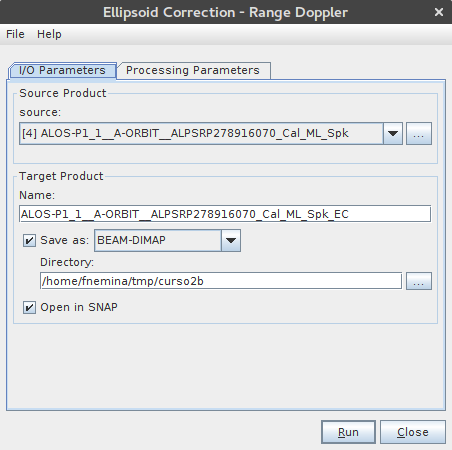
\includegraphics[width=0.35\textwidth]{fig:elipsoide1.png}}
        \hspace{1cm}
        \subfloat[Processing parameters]{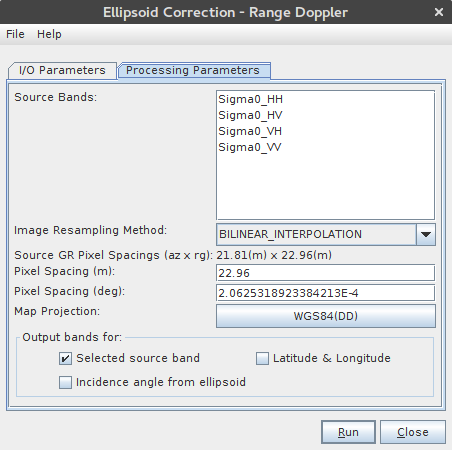
\includegraphics[width=0.35\textwidth]{fig:elipsoide2.png}}
        \caption{Proyección de un producto SAR sobre el elipsoide.}
        \label{fig:elipsoide}
    \end{figure}

\subsection{Modelo de elevación digital - GTC}

Para proyectar la imagen sobre un modelo de elevación digital vaya al menú \menu{Radar>Geometric>Terrain Correction>Range Doppler Terrain Correction}. Seleccione la imagen
\begin{center} \texttt{ALOS-P1\_1\_\_A-ORBIT\_\_ALPSRP278916070\_Cal\_ML\_DSk}
  \end{center}
  y en \menu{processing parameters} destilde la opción \emph{Mask out areas without elevation} (Figura \ref{fig:gtc}).



{\bf Importante:} Al realizar la proyección sobre un DEM el SNAP lo descarga automaticamente. Esto puede tomar varios minutos dependiendo de su conexión.

\begin{figure}[h!]
    \centering
    \subfloat[I/O Parameters]{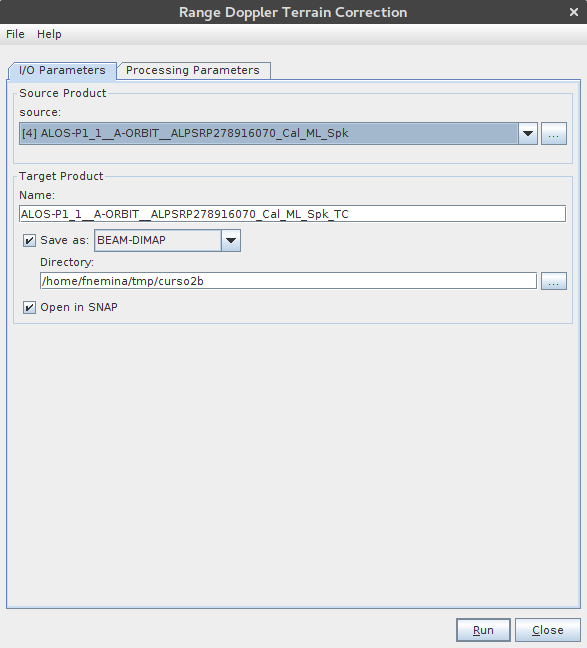
\includegraphics[width=0.35\textwidth]{fig:gtc1.png}}
    \hspace{1cm}
    \subfloat[Processing parameters]{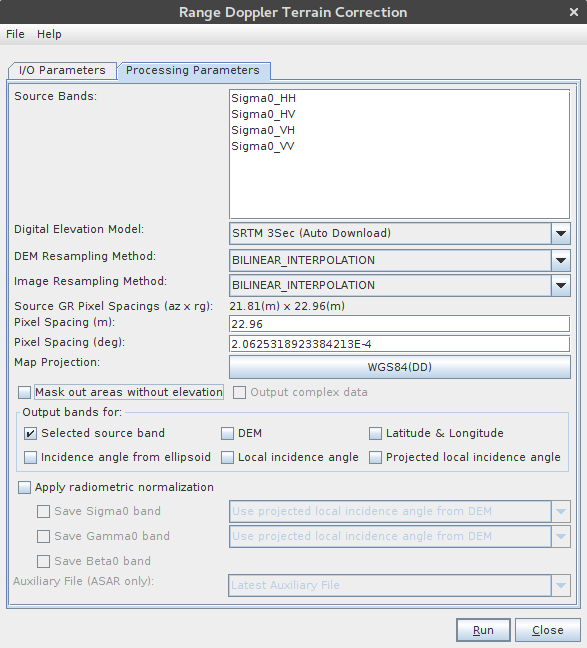
\includegraphics[width=0.35\textwidth]{fig:gtc2.png}}
    \caption{Proyección de un producto SAR sobre un DEM.}
    \label{fig:gtc}
\end{figure}

\section{Conversión a dB}

Puede convertir la imagen a dB haciendo click derecho sobre la banda y seleccionando la opción \menu{Linear to/from dB}.

Convierta a dB la banda \texttt{sigma\_0\_HH} y explore visualmente el resultado. Conviene siempre explorar las imagenes en dB pues es una medida más natural para nuestro ojo.

\section{Preguntas para debate}

\begin{que}
    Observe y compare la banda \texttt{sigma\_0\_HH} de la imagen con y sin filtro.
\end{que}

\begin{que}
    Compare visualmente las imágenes GTC y GEC obtenidas por los métodos anteriores para la banda \texttt{sigma\_0\_HH\_dB}. ¿Qué sucede con las montañas? ¿Hacia donde parecen estar inclinadas?
\end{que}

\begin{que}
    ¿Por qué las montañas parecen mas brillantes de un lado que del otro?
\end{que}

\begin{que}
    Obtenga los valores de dB para las coberturas de agua, urbano y bosque para la banda \texttt{sigma\_0\_HH\_dB}.
\end{que}

\begin{que}
    Dentro del Canal de Beagle encontrará un punto muy brillante cerca de la ciudad de Ushuahia. ¿A qué se debe este punto? ¿Qué aplicación le encuentra a las imágenes SAR sobre el agua?
\end{que}

Estas preguntas no serán evaluadas. Su objetivo es discutirlas en el foro de sonsultas e intercambio de la clase.
